% Provenance (never printed): cycle 4 SVT, "La planete Terre": volcanic
% activity, its products and its link with plate boundaries; natural hazards
% and their monitoring; see sources/book1/PROVENANCE.md. Book 1, grade 7,
% chapter 2.
% Vocabulary guard: "magma" first allowed here; "sediment" not before g7.4;
% "subduction zone" is never a term here (gloss: "where one plate sinks under
% another"); "hotspot track" is Book 2's; lahars are called mudflows.
\chapter{البراكين}\label{ch:g7:volcanoes}

في 17~مايو 1980، وقف جيولوجي على مرتفع يبعد عشرة كيلومترات عن \omterm{def:g1:landscapes-around-us:landform}{جبل}
سانت~هيلينز، في الشمال الغربي من الولايات المتحدة، والتقط الصورة
التي على اليمين أدناه: مخروط أملس مكسو \omterm{def:g4:clouds-rain-snow:precipitation}{بالثلج}، من أجمل \omterm{def:g1:landscapes-around-us:landform}{جبال}
البلاد. وطوال شهرين كان \omterm{def:g1:landscapes-around-us:landform}{الجبل} يرتجف، وكان سفحه
الشمالي ينتفخ نحو الخارج كالبالون. وفي صباح اليوم التالي، في الساعة
\babelsublr{8:32}، هزّه \omterm{def:g4:volcanoes-earthquakes-first-look:earthquake}{زلزال} صغير. فانزلق السفح المنتفخ كله،
وانفجر \omterm{def:g4:volcanoes-earthquakes-first-look:volcano}{البركان} جانبيًا. وحين أمكن تصوير المرتفع نفسه
من جديد، في سبتمبر، كان \omterm{def:g1:landscapes-around-us:landform}{الجبل} يبدو كما في الصورة التي على اليسار.

\begin{omfigure}
\begin{minipage}[b]{0.495\linewidth}\centering
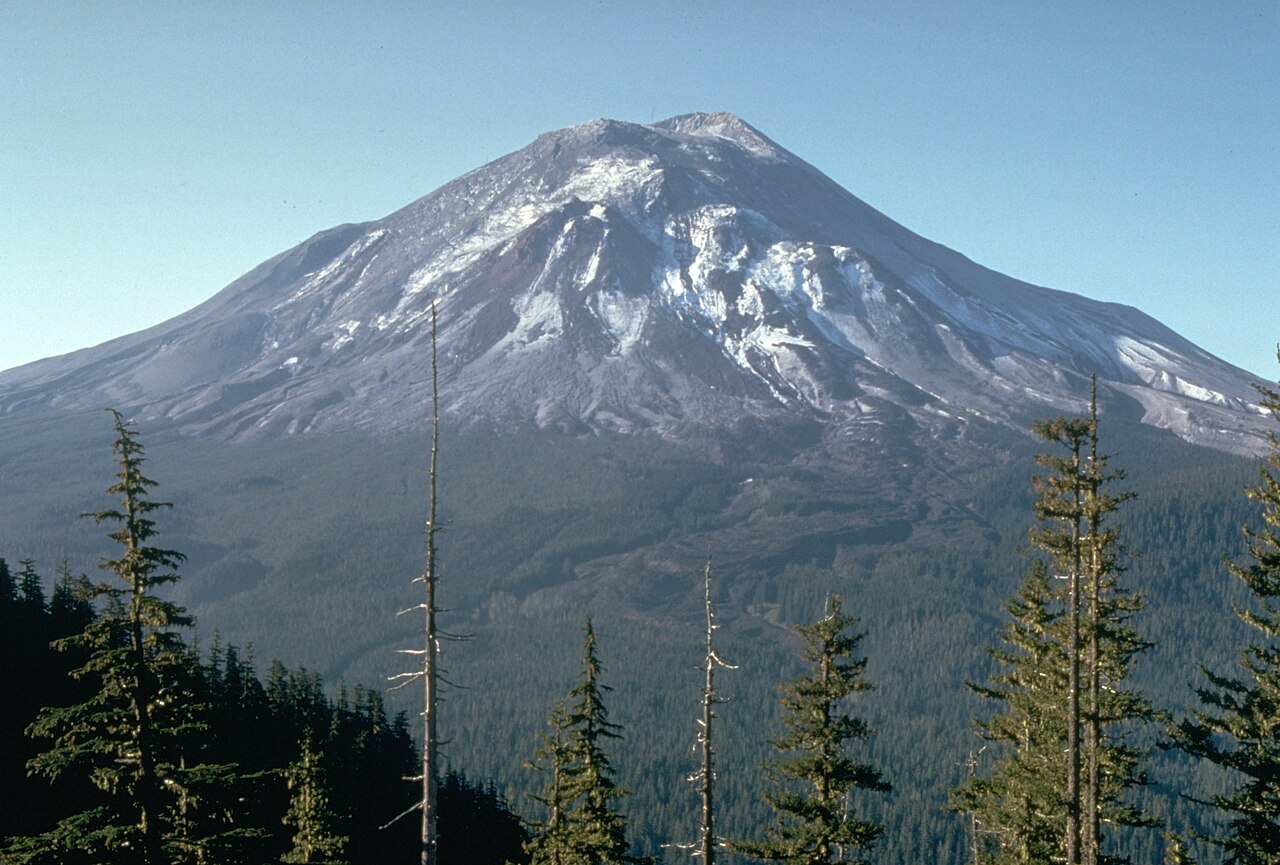
\includegraphics[width=\linewidth]{images/book1/g7-msh-before.jpg}

{\small 17 مايو 1980، اليوم السابق.}
\end{minipage}\hfill
\begin{minipage}[b]{0.495\linewidth}\centering
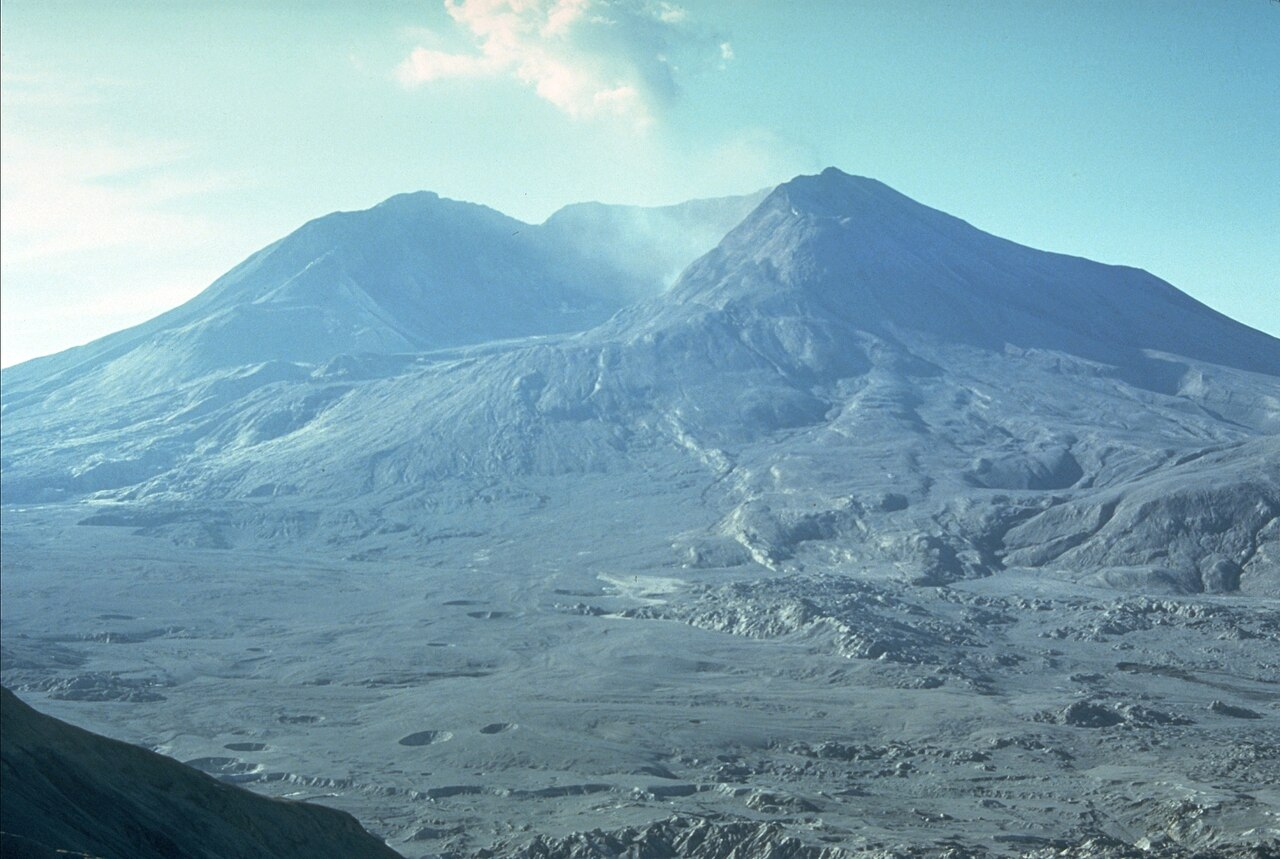
\includegraphics[width=\linewidth]{images/book1/g7-msh-after.jpg}

{\small 10 سبتمبر 1980.}
\end{minipage}

{\small \omterm{def:g1:landscapes-around-us:landform}{جبل} سانت~هيلينز كما يُرى من مرتفع جونستون، قبل
\omterm{def:g4:volcanoes-earthquakes-first-look:eruption}{ثوران} 18~مايو 1980 وبعده. فقد زالت القمة والسفح الشمالي كله؛ وحلّت
محلهما \omterm{def:g7:volcanoes:vent}{فوهة} مفتوحة نحو الشمال. الصورتان: هاري
غليكن، هيئة المسح الجيولوجي الأمريكية (ملك عام، عبر ويكيميديا كومنز).}
% ledger: commons:msh-before, commons:msh-after, usgs:msh-lead-up, usgs:msh-may18
\label{fig:g7:volcanoes:st-helens}
\end{omfigure}

في هذا الفصل نفتح \omterm{def:g4:volcanoes-earthquakes-first-look:volcano}{بركانًا} لنرى ما الذي يدفع \omterm{def:g4:volcanoes-earthquakes-first-look:eruption}{الثوران}؛ ونكتشف
لماذا تصب بعض \omterm{def:g4:volcanoes-earthquakes-first-look:volcano}{البراكين} أنهارًا هادئة من \omterm{def:g4:volcanoes-earthquakes-first-look:eruption}{الحمم} بينما تفجّر \omterm{def:g4:volcanoes-earthquakes-first-look:volcano}{براكين} أخرى
نفسها؛ ثم ننظر إلى \omterm{def:g3:continents-and-oceans:world-map}{خريطة العالم} من جديد، لنرى أين تقع
\omterm{def:g4:volcanoes-earthquakes-first-look:volcano}{البراكين} ولماذا.

\begin{recall}
\emph{\omterm{def:g4:volcanoes-earthquakes-first-look:volcano}{البركان}} مكان يخرج فيه \omterm{def:g3:stones-pebbles-sand:rock}{صخر} منصهر من أعماق الأرض
إلى السطح، وهو أيضًا التل أو \omterm{def:g1:landscapes-around-us:landform}{الجبل} الذي يبنيه هناك.
وأثناء \emph{\omterm{def:g4:volcanoes-earthquakes-first-look:eruption}{الثوران}} يقذف \omterm{def:g4:volcanoes-earthquakes-first-look:eruption}{حممًا} ورمادًا وغازًا
(\cref{ch:g4:volcanoes-earthquakes-first-look}). وتحت \omterm{def:g6:inside-the-earth:layers}{القشرة}، يتكون
\omterm{def:g6:inside-the-earth:layers}{الوشاح} من \omterm{def:g3:stones-pebbles-sand:rock}{صخر} حار صلب، مع أنه يستطيع أن يزحف ببطء
شديد (\cref{ch:g6:inside-the-earth}). والبازلت والغرانيت \omterm{def:g6:rocks-and-minerals:rock-families}{صخور
نارية}: تتكون حين يبرد \omterm{def:g3:stones-pebbles-sand:rock}{الصخر} المنصهر ويتصلب
(\cref{ch:g6:rocks-and-minerals}). والغلاف الخارجي للأرض مكسَّر
\omterm{def:g7:plate-tectonics:plate}{صفائح} تتحرك بضعة سنتيمترات في السنة؛ وحوافها هي \omterm{def:g7:plate-tectonics:plate-boundary}{حدود
الصفائح} (\cref{ch:g7:plate-tectonics}).
\end{recall}

\section{داخل البركان}

\omterm{def:g6:inside-the-earth:layers}{الوشاح} صلب. ومع ذلك ففي أماكن قليلة، في الأعماق تحت السطح، ينصهر جزء
صغير من \omterm{def:g3:stones-pebbles-sand:rock}{الصخر}. \omterm{def:g3:stones-pebbles-sand:rock}{والصخر} المنصهر أخف من \omterm{def:g3:stones-pebbles-sand:rock}{الصخر} الصلب
\omterm{def:g2:water-on-earth:ocean}{المحيط} به، فيصعد ببطء، شاقًّا طريقه عبر الشقوق، كما تصعد قطرة
زيت عبر الماء.
% ledger: usgs:hawaii-hotspot (magma lighter than the surrounding rock, rises)

\begin{definition}[الصهارة]\label{def:g7:volcanoes:magma}
\emph{الصهارة}\index{صهارة} \omterm{def:g3:stones-pebbles-sand:rock}{صخر} منصهر تحت الأرض. وهي سائل حار
قد يحمل أيضًا بلورات، وتذوب فيه غازات مثل بخار
الماء وثاني أكسيد الكربون. والصهارة التي تخرج إلى السطح تسمى
\omterm{def:g4:volcanoes-earthquakes-first-look:eruption}{حممًا}؛ وحين تخرج، تفقد معظم غازها.
\end{definition}

كثيرًا ما تتوقف \omterm{def:g7:volcanoes:magma}{الصهارة} الصاعدة في طريقها، على بعد بضعة كيلومترات تحت السطح،
حيث تتجمع في جيب كبير. وهناك تنتظر، أحيانًا
قرونًا، قبل أن يُفرغ \omterm{def:g4:volcanoes-earthquakes-first-look:eruption}{ثوران} جزءًا منها.

\begin{definition}[حجرة الصهارة]\label{def:g7:volcanoes:magma-chamber}
\emph{حجرة الصهارة}\index{حجرة الصهارة} فراغ كبير في \omterm{def:g3:stones-pebbles-sand:rock}{الصخور}
تحت \omterm{def:g4:volcanoes-earthquakes-first-look:volcano}{البركان}، على عمق بضعة كيلومترات، تتجمع فيه \omterm{def:g7:volcanoes:magma}{الصهارة} قبل
\omterm{def:g4:volcanoes-earthquakes-first-look:eruption}{الثوران}.
\end{definition}

\begin{definition}[المنفذ والفوهة]\label{def:g7:volcanoes:vent}
\emph{المنفذ}\index{منفذ} فتحة في السطح تخرج منها \omterm{def:g7:volcanoes:magma}{الصهارة}
والغاز والرماد. و\emph{الفوهة}\index{فوهة} تجويف على شكل
وعاء حول المنفذ، يقع عادة في قمة \omterm{def:g4:volcanoes-earthquakes-first-look:volcano}{البركان}.
\end{definition}

\begin{omfigure}
\begin{tikzpicture}[font=\small, x=1cm, y=1cm]
  % rocks below the volcano
  \fill[brown!25] (-6,-4.2) rectangle (6,0);
  \draw[brown!50] (-6,-1.4) -- (6,-1.4) (-6,-2.8) -- (6,-2.8);
  % the cone, built of layers of lava (dark) and ash (light)
  \fill[black!45] (-5.2,0) -- (-0.75,3.4) -- (0.75,3.4) -- (5.2,0) -- cycle;
    % layers dipping outwards, parallel to the flanks (slope 3.4/4.45)
  \foreach \k/\c in {0/black!25, 2/black!25, 4/black!25} {
    \pgfmathsetmacro{\xa}{-5.2+0.8*\k}\pgfmathsetmacro{\xb}{-5.2+0.8*(\k+1)}
    \pgfmathsetmacro{\ya}{(-0.18-\xa)*3.4/4.45}\pgfmathsetmacro{\yb}{(-0.18-\xb)*3.4/4.45}
    \fill[\c] (\xa,0) -- (-0.18,\ya) -- (-0.18,\yb) -- (\xb,0) -- cycle;
    \fill[\c] (-\xa,0) -- (0.18,\ya) -- (0.18,\yb) -- (-\xb,0) -- cycle;
  }
  % the crater at the top
  \fill[white] (-0.75,3.4) -- (-0.3,2.95) -- (0.3,2.95) -- (0.75,3.4) -- cycle;
  \draw[black!70] (-0.75,3.4) -- (-0.3,2.95) -- (0.3,2.95) -- (0.75,3.4);
  % magma chamber and the pipe up to the vent
  \fill[orange!85!red] (0,-3.0) ellipse (2.1 and 0.75);
  \fill[orange!85!red] (-0.18,-2.4) rectangle (0.18,2.98);
  % a side branch to a small side vent
  \fill[orange!85!red] (0.1,0.6) -- (2.55,1.5) -- (2.62,1.33) -- (0.1,0.25) -- cycle;
  % lava flow down the right flank, from the side vent
  \fill[orange!95!red] (2.5,1.45) .. controls (3.2,1.0) and (3.7,0.5) .. (4.6,0.08)
    -- (4.0,0.05) .. controls (3.3,0.4) and (2.9,0.8) .. (2.45,1.25) -- cycle;
  % ash column and gas
    \fill[black!22] (-0.3,3.0) -- (0.3,3.0) -- (0.45,3.9) -- (-0.45,3.9) -- cycle;
  \foreach \x/\y/\r in {0/3.95/0.45, -0.45/4.55/0.55, 0.45/4.6/0.5, -0.15/5.2/0.6,
                        0.6/5.3/0.5, -0.8/5.15/0.45, 0.15/5.8/0.55}
    \fill[black!22] (\x,\y) circle (\r);
  % labels
  \node[anchor=west] at (2.1,5.3) {عمود الرماد والغاز};
  \draw[black!60] (2.05,5.3) -- (1.05,5.2);
  \node[anchor=west] at (2.0,3.3) {الفوهة};
  \draw[black!60] (1.95,3.3) -- (0.6,3.2);
  \node[anchor=east] at (-2.0,3.8) {المنفذ الرئيسي};
  \draw[black!60] (-1.95,3.75) -- (-0.1,3.0);
  \node[anchor=west] at (4.2,1.6) {منفذ جانبي};
  \draw[black!60] (4.15,1.6) -- (2.65,1.45);
  \node[anchor=west] at (4.5,0.55) {سيل حمم};
  \draw[black!60] (4.45,0.55) -- (3.9,0.4);
  \node[anchor=east, align=right] at (-3.0,1.75) {طبقات من\\الحمم والرماد};
  \draw[black!60] (-2.95,1.6) -- (-2.2,1.1);
  \node[anchor=west, align=left] at (0.55,-0.9) {صهارة تصعد\\في قناة};
  \draw[black!60] (0.5,-0.9) -- (0.2,-0.9);
  \node[anchor=west] at (2.3,-3.0) {حجرة الصهارة};
  \draw[black!60] (2.25,-3.0) -- (1.7,-3.0);
  \node[anchor=west, align=left, font=\footnotesize] at (-5.9,-3.7) {على عمق بضعة كيلومترات};
  \draw[black!60, <->] (-4.3,0) -- (-4.3,-3.0);
\end{tikzpicture}

{\small \omterm{def:g4:volcanoes-earthquakes-first-look:volcano}{بركان} مقطوع (رسم بلا مقياس رسم). تتجمع \omterm{def:g7:volcanoes:magma}{الصهارة} في
\omterm{def:g7:volcanoes:magma-chamber}{حجرة الصهارة} وتصعد عبر قناة إلى \omterm{def:g7:volcanoes:vent}{المنفذ} الرئيسي، في قاع
\omterm{def:g7:volcanoes:vent}{الفوهة}؛ ويصل فرع منها إلى \omterm{def:g7:volcanoes:vent}{منفذ} جانبي على السفح. وكل \omterm{def:g4:volcanoes-earthquakes-first-look:eruption}{ثوران} يضيف
طبقة من \omterm{def:g4:volcanoes-earthquakes-first-look:eruption}{الحمم} أو من الرماد إلى المخروط.}
\label{fig:g7:volcanoes:cutaway}
\end{omfigure}

إذن \omterm{def:g3:stones-pebbles-sand:rock}{للصخر} المنصهر نفسه اسمان. فهو تحت الأرض \emph{\omterm{def:g7:volcanoes:magma}{صهارة}}؛ وما إن
يخرج من \omterm{def:g7:volcanoes:vent}{منفذ} حتى يصير \emph{\omterm{def:g4:volcanoes-earthquakes-first-look:eruption}{حممًا}}. والفرق ليس مجرد
مسألة ألفاظ: \omterm{def:g7:volcanoes:magma}{فالصهارة} لا تزال تحتفظ بغازها، أما \omterm{def:g4:volcanoes-earthquakes-first-look:eruption}{الحمم} فقد فقدت معظمه
في الهواء. وسنرى أن هذا الغاز هو الذي يحدد نوع \omterm{def:g4:volcanoes-earthquakes-first-look:eruption}{الثوران} الذي
يحدث في \omterm{def:g4:volcanoes-earthquakes-first-look:volcano}{البركان}.

ما درجة حرارتها؟ يقيس علماء مرصد \omterm{def:g4:volcanoes-earthquakes-first-look:volcano}{براكين} هاواي
\omterm{def:g4:volcanoes-earthquakes-first-look:eruption}{الحمم} حين تخرج من منافذ كيلاويا، أحد \omterm{def:g4:volcanoes-earthquakes-first-look:volcano}{براكين}
هاواي: نحو \qty{1170}{\degreeCelsius}. \omterm{def:g3:stones-pebbles-sand:rock}{والصخر} الحار يتوهج، ولون
التوهج يتوقف على درجة حرارته: فكاميرات خاصة تقرأ درجة حرارة
سيل \omterm{def:g4:volcanoes-earthquakes-first-look:eruption}{الحمم} من بعيد بقياس ألوان توهجه. وحتى العين
تكوّن فكرة تقريبية، كما يبيّن الجدول.
% ledger: usgs:kilauea-temp, usgs:pyrometer

\begin{center}
\small
\begin{tabular}{|l|c|}
\hline
\textbf{لون \omterm{def:g3:stones-pebbles-sand:rock}{الصخر} المتوهج} & \textbf{درجة الحرارة} \\
\hline
أصفر & من نحو 1000 إلى \qty{1200}{\degreeCelsius} \\
برتقالي & من نحو 800 إلى \qty{1000}{\degreeCelsius} \\
أحمر & من نحو 600 إلى \qty{800}{\degreeCelsius} \\
\hline
\end{tabular}
\end{center}
% ledger: usgs:kilauea-temp

\begin{remark}[قشرة تبرد في ثانية]\label{rem:g7:volcanoes:skin}
% ledger: usgs:kilauea-temp
حين تلامس \omterm{def:g4:volcanoes-earthquakes-first-look:eruption}{الحمم} الهواء أول مرة، يبرد سطحها بمئات الدرجات
في كل ثانية: فتتكون في الحال \omterm{def:g6:inside-the-earth:layers}{قشرة} داكنة على \omterm{def:g3:stones-pebbles-sand:rock}{الصخر} المتوهج. وتحت
\omterm{def:g6:inside-the-earth:layers}{القشرة} تبقى \omterm{def:g4:volcanoes-earthquakes-first-look:eruption}{الحمم} حارة مدة طويلة. ففي هاواي، جرت \omterm{def:g4:volcanoes-earthquakes-first-look:eruption}{الحمم} في
أنفاق تحت سقفها المتصلب نفسه مسافة \qty{10}{km}، من \omterm{def:g7:volcanoes:vent}{منفذ} إلى
\omterm{def:g2:water-on-earth:ocean}{البحر}، ومع ذلك بلغت الشاطئ وحرارتها نحو \qty{1140}{\degreeCelsius}: أي أبرد
بنحو 30~درجة فقط مما كانت عند \omterm{def:g7:volcanoes:vent}{المنفذ}.
\end{remark}

\begin{omfigure}
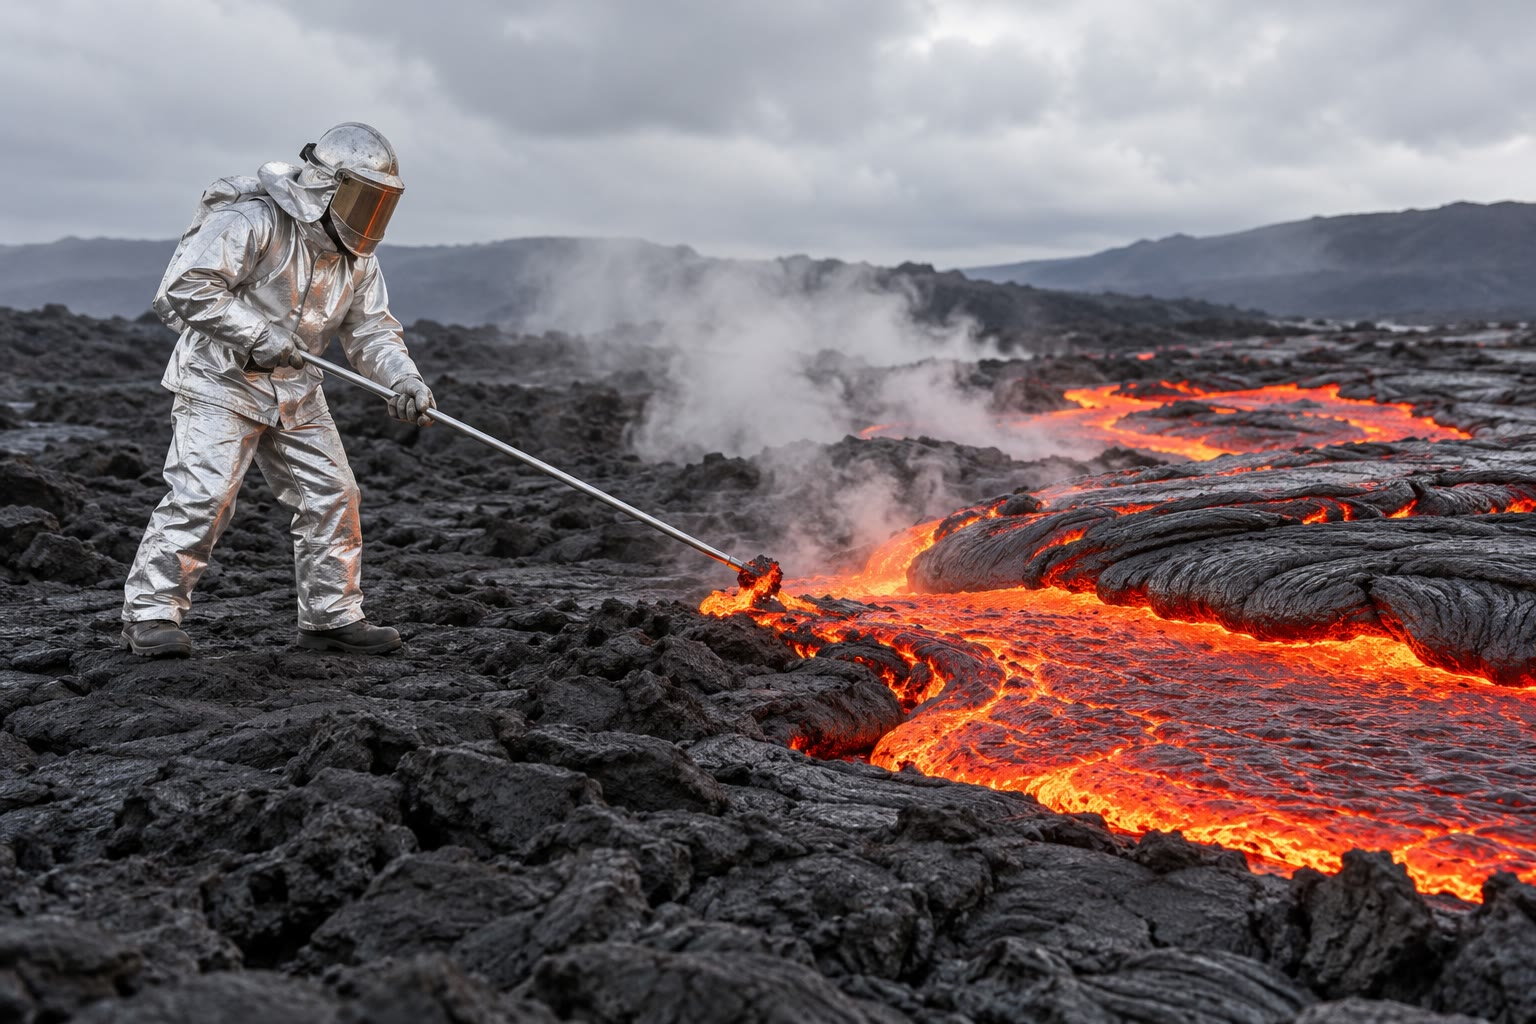
\includegraphics[width=0.6\linewidth]{images/book1/ai/g7-volcanologist.jpg}

{\small عالم \omterm{def:g4:volcanoes-earthquakes-first-look:volcano}{براكين} في بدلة عاكسة للحرارة يأخذ عينة من \omterm{def:g4:volcanoes-earthquakes-first-look:eruption}{الحمم}
بعمود فولاذي طويل (رسم بالذكاء الاصطناعي لمشهد عام).
ولا يقترب من \omterm{def:g4:volcanoes-earthquakes-first-look:eruption}{الحمم} الجارية إلا العلماء المدرَّبون، بمثل هذه المعدات؛
أما الآخرون فيشاهدون من حيث تسمح السلطات.}
\label{fig:g7:volcanoes:volcanologist}
\end{omfigure}

\section{طريقتان للثوران}

فجّر \omterm{def:g1:landscapes-around-us:landform}{جبل} سانت~هيلينز نفسه. أما \omterm{def:g4:volcanoes-earthquakes-first-look:volcano}{براكين} هاواي، فعلى
العكس، تصب عادة \omterm{def:g4:volcanoes-earthquakes-first-look:eruption}{حممًا} تجري نازلة على منحدراتها.
ويصنّف الجيولوجيون \omterm{def:g4:volcanoes-earthquakes-first-look:eruption}{الثورانات} في نوعين.

\begin{definition}[الثوران الانسيابي والثوران الانفجاري]\label{def:g7:volcanoes:eruption-types}
في \emph{الثوران الانسيابي}\index{ثوران انسيابي} تخرج \omterm{def:g7:volcanoes:magma}{الصهارة}
بهدوء \omterm{def:g4:volcanoes-earthquakes-first-look:eruption}{حممًا}، تجري بعيدًا عن \omterm{def:g7:volcanoes:vent}{المنفذ}، أحيانًا كيلومترات،
أو تندفع إلى الأعلى في نوافير من القطرات المتوهجة. وفي \emph{الثوران
الانفجاري}\index{ثوران انفجاري} تتمزق \omterm{def:g7:volcanoes:magma}{الصهارة} قطعًا بفعل
غازها: فيُقذف عمود من الرماد والغاز وكتل \omterm{def:g3:stones-pebbles-sand:rock}{الصخر} عاليًا في
السماء.
\end{definition}

\begin{omfigure}
\begin{minipage}[t]{0.49\linewidth}\centering
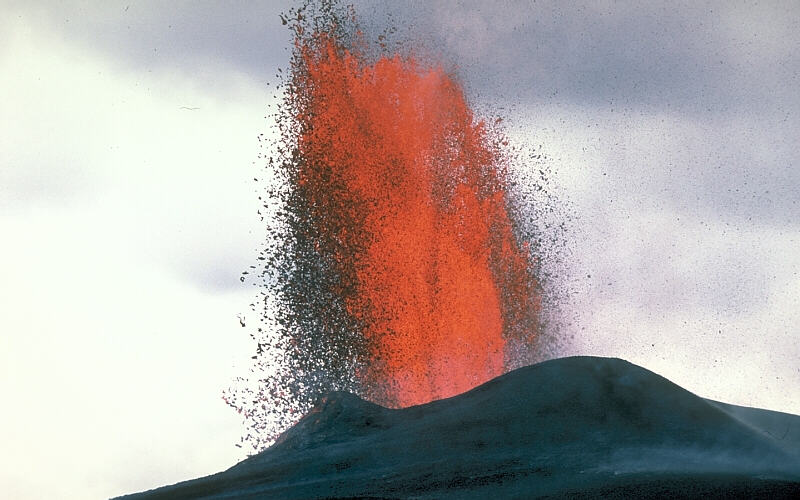
\includegraphics[height=4.5cm]{images/book1/g7-lava-fountain.jpg}

{\small انسيابي: نافورة \omterm{def:g4:volcanoes-earthquakes-first-look:eruption}{حمم} في كيلاويا، هاواي، 1983.
الصورة: ج.~د.~غريغز، هيئة المسح الجيولوجي الأمريكية.}
\end{minipage}\hfill
\begin{minipage}[t]{0.49\linewidth}\centering
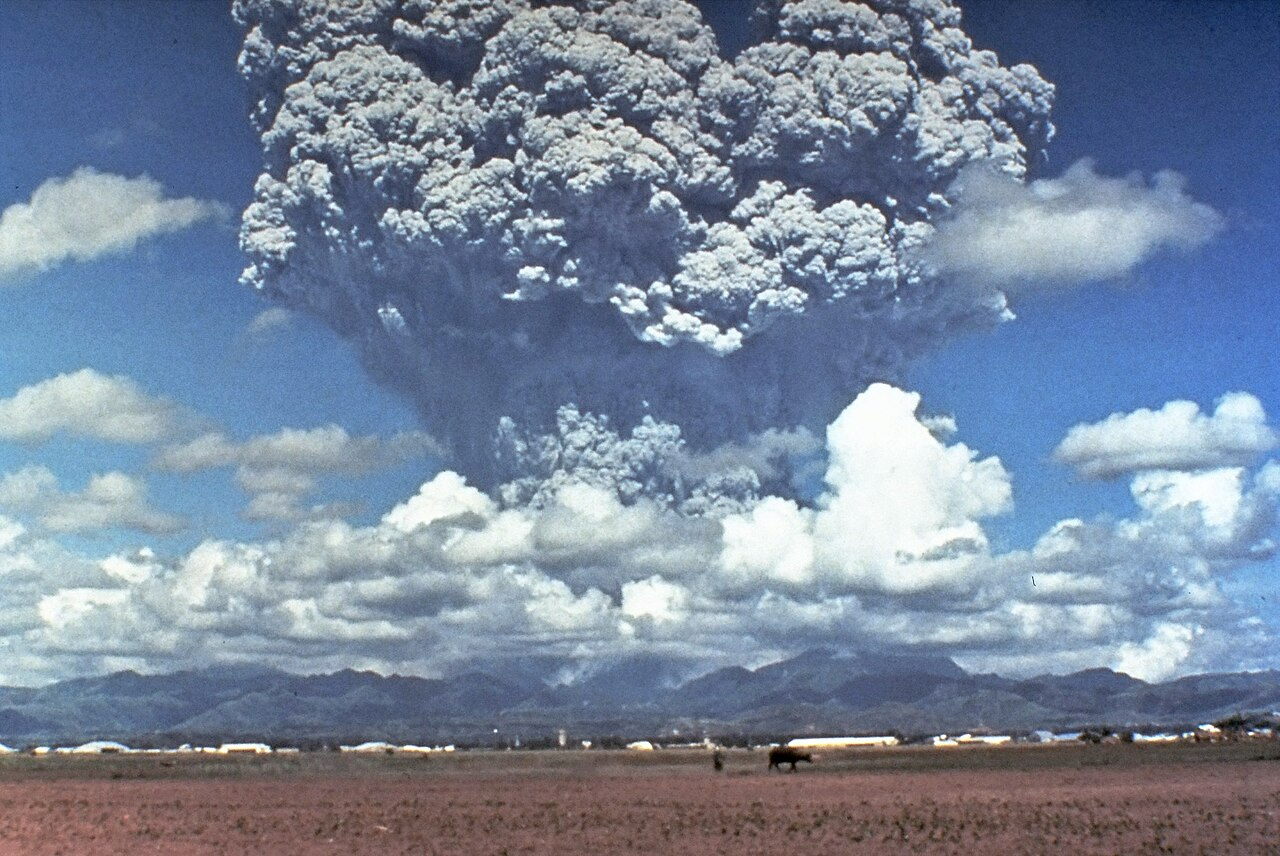
\includegraphics[height=4.5cm]{images/book1/g7-pinatubo.jpg}

{\small انفجاري: عمود \omterm{def:g4:volcanoes-earthquakes-first-look:eruption}{ثوران} \omterm{def:g1:landscapes-around-us:landform}{جبل} بيناتوبو، الفلبين،
12~يونيو 1991. الصورة: ديف هارلو، هيئة المسح الجيولوجي الأمريكية.}
\end{minipage}\par\medskip


{\small الصورتان كلتاهما ملك عام (عبر ويكيميديا
كومنز).}
% ledger: commons:lava-fountain, commons:pinatubo
\label{fig:g7:volcanoes:two-photos}
\end{omfigure}

ما الذي يصنع الفرق؟ أمران: مدى سيولة \omterm{def:g7:volcanoes:magma}{الصهارة}، ومقدار
الغاز الذي تحمله.

\textbf{سائلة أم لزجة.} بعض \omterm{def:g7:volcanoes:magma}{الصهارة} سائلة، تكاد تكون كالعسل الدافئ: وهذه
حال \omterm{def:g7:volcanoes:magma}{الصهارة} التي تبرد فتصير بازلتًا داكنًا، كما في هاواي. \omterm{def:g7:volcanoes:magma}{وصهارة}
أخرى كثيفة لزجة، كالعسل البارد أو معجون الأسنان. فعبر \omterm{def:g7:volcanoes:magma}{الصهارة}
السائلة، تصعد فقاعات الغاز بسهولة وتفلت عند السطح، القليل منها في كل مرة.
أما في \omterm{def:g7:volcanoes:magma}{الصهارة} اللزجة فتبقى الفقاعات محبوسة.

\textbf{غاز قليل أم كثير.} قنينة الماء الغازي تحمل كثيرًا من الغاز
الذائب في الماء، يبقيه هناك الضغط داخل القنينة
المغلقة؛ فلا تراه. افتح القنينة فينخفض الضغط: فتظهر الفقاعات
في كل مكان، وإذا كانت القنينة قد رُجّت، اندفعت الرغوة إلى الخارج.
\omterm{def:g7:volcanoes:magma}{والصهارة} في أعماق الأرض تحمل هي أيضًا غازًا ذائبًا تحت ضغط عالٍ. فحين
تصعد، ينخفض الضغط ويخرج الغاز من المحلول فقاعات.
% ledger: usgs:volcanic-gases

لنجمع الأمرين. \omterm{def:g7:volcanoes:magma}{الصهارة} السائلة القليلة الغاز تترك فقاعاتها تفلت
وتخرج \omterm{def:g4:volcanoes-earthquakes-first-look:eruption}{حممًا} جارية: فيكون \omterm{def:g4:volcanoes-earthquakes-first-look:eruption}{الثوران} انسيابيًا. \omterm{def:g7:volcanoes:magma}{والصهارة} اللزجة المليئة
بالغاز تحتفظ بفقاعاتها حتى تنتفخ إلى حد أن تمزق \omterm{def:g7:volcanoes:magma}{الصهارة}
مِزقًا: فيكون \omterm{def:g4:volcanoes-earthquakes-first-look:eruption}{الثوران} انفجاريًا. ومِزق \omterm{def:g7:volcanoes:magma}{الصهارة} المزبدة تتجمد
في الهواء رمادًا وخفافًا، والخفاف \omterm{def:g3:stones-pebbles-sand:rock}{صخر} مليء بالفقاعات إلى حد أنه يستطيع أن
يطفو.

\begin{example}[بيناتوبو، 1991: المشروب الغازي الذي فقد غازه والآخر المرجوج]\label{ex:g7:volcanoes:pinatubo}
% ledger: usgs:pinatubo-1991
في يونيو~1991 وصلت أول \omterm{def:g7:volcanoes:magma}{صهارة} إلى سطح \omterm{def:g1:landscapes-around-us:landform}{جبل} بيناتوبو، في
الفلبين. وكانت قد فقدت في طريقها إلى الأعلى معظم غازها، «كقنينة
مشروب غازي فقد غازه»، على حد تعبير العلماء الذين كانوا يراقبون.
فنزّت ببطء وتكدست كومةً فوق \omterm{def:g7:volcanoes:vent}{المنفذ}: بلا انفجار.
ثم في 12~يونيو، وصلت إلى السطح \omterm{def:g7:volcanoes:magma}{صهارة} لا تزال مليئة بالغاز
وانفجرت --- وهو العمود الذي في الصورة أعلاه. وفي 15~يونيو، وصلت \omterm{def:g7:volcanoes:magma}{صهارة} أغنى
بالغاز أيضًا، فشهد \omterm{def:g4:volcanoes-earthquakes-first-look:volcano}{البركان} واحدًا من أكبر \omterm{def:g4:volcanoes-earthquakes-first-look:eruption}{ثورانات}
القرن العشرين: إذ قذف أكثر من خمسة كيلومترات مكعبة من
\omterm{def:g3:stones-pebbles-sand:rock}{الصخر} والرماد، وارتفعت \omterm{def:g4:clouds-rain-snow:cloud}{سحابة} رماده \qty{35}{km}، وانهارت قمة
\omterm{def:g1:landscapes-around-us:landform}{الجبل} في تجويف عرضه \qty{2.5}{km}. \omterm{def:g4:volcanoes-earthquakes-first-look:volcano}{البركان} نفسه،
والأسبوع نفسه: والغاز هو الذي صنع الفرق.
\end{example}

شكل \omterm{def:g4:volcanoes-earthquakes-first-look:volcano}{البركان} يحفظ ذاكرة ثوراناته. \omterm{def:g4:volcanoes-earthquakes-first-look:eruption}{فالحمم} السائلة تجري
بعيدًا قبل أن تتصلب، فتبني طبقة بعد طبقة جبلًا عريضًا ذا
منحدرات لطيفة، على شكل ترس محارب ملقى على الأرض: إنه
\emph{\omterm{def:g4:volcanoes-earthquakes-first-look:volcano}{البركان} الدرعي}. وماونا لوا، في هاواي، واحد منها. أما \omterm{def:g4:volcanoes-earthquakes-first-look:eruption}{الحمم} اللزجة والرماد فتتكدس
قرب \omterm{def:g7:volcanoes:vent}{المنفذ}، في مخروط شديد الانحدار مكوَّن من طبقات من \omterm{def:g4:volcanoes-earthquakes-first-look:eruption}{الحمم}
والرماد: إنه \emph{البركان الطبقي} (\emph{ستراتا} تعني الطبقات). \omterm{def:g1:landscapes-around-us:landform}{وجبل} سانت~هيلينز
وبيناتوبو اثنان منها.

\begin{omfigure}
\begin{tikzpicture}[font=\small, x=1cm, y=1cm]
  % --- left: effusive, a shield
  \begin{scope}
    \fill[brown!25] (-3.3,-1.2) rectangle (3.3,0);
    \fill[black!50] (-3.3,0) .. controls (-2.0,0.45) and (-1.0,1.0) .. (-0.35,1.25)
      -- (0.35,1.25) .. controls (1.0,1.0) and (2.0,0.45) .. (3.3,0) -- cycle;
    \fill[orange!85!red] (-0.12,-1.2) rectangle (0.12,1.25);
    % fountain
    \foreach \a in {-25,-12,0,12,25}
      \draw[orange!90!red, line width=0.9pt] (0,1.25) .. controls ({0.4*sin(\a)},2.2) .. ({1.0*sin(\a)},1.6);
    % lava flows far down the gentle slopes
    \draw[orange!95!red, line width=2.2pt, line cap=round] (0.3,1.22) .. controls (1.2,0.95) and (2.1,0.45) .. (3.1,0.08);
    \draw[orange!95!red, line width=2.2pt, line cap=round] (-0.3,1.22) .. controls (-1.3,0.95) and (-2.2,0.45) .. (-3.0,0.1);
    \node[font=\small\bfseries] at (0,4.3) {انسيابي};
    \node[align=center, font=\footnotesize] at (0,-1.75) {صهارة سائلة وغاز قليل\\الحمم تجري بعيدًا؛ ودرع عريض};
    \node[anchor=west, font=\footnotesize] at (1.2,1.9) {نافورة حمم};
    \draw[black!60] (1.15,1.9) -- (0.6,1.75);
    \node[anchor=west, font=\footnotesize, align=left] at (1.9,1.2) {سيول حمم\\طويلة};
    \draw[black!60] (1.85,1.05) -- (1.5,0.82);
  \end{scope}
  % --- right: explosive, a steep cone
  \begin{scope}[xshift=7.4cm]
    \fill[brown!25] (-3.3,-1.2) rectangle (3.3,0);
    \fill[black!45] (-2.3,0) -- (-0.4,2.2) -- (0.4,2.2) -- (2.3,0) -- cycle;
    \fill[orange!85!red] (-0.12,-1.2) rectangle (0.12,2.2);
    \foreach \x/\y/\r in {0/2.6/0.35, -0.3/3.05/0.4, 0.3/3.1/0.38, 0/3.5/0.45, -0.45/3.55/0.32, 0.45/3.6/0.32}
      \fill[black!28] (\x,\y) circle (\r);
    % pyroclastic flow down the flank
    \fill[black!30] (0.45,2.1) .. controls (1.0,1.5) and (1.6,0.7) .. (2.9,0.05)
      -- (2.2,0.05) .. controls (1.4,0.45) and (0.9,1.2) .. (0.35,1.95) -- cycle;
    \node[font=\small\bfseries] at (0,4.3) {انفجاري};
    \node[align=center, font=\footnotesize] at (0,-1.75) {صهارة لزجة وغاز كثير\\عمود رماد؛ ومخروط شديد الانحدار};
    \node[anchor=west, font=\footnotesize] at (0.9,3.4) {عمود رماد};
    \draw[black!60] (0.85,3.4) -- (0.7,3.4);
    \node[anchor=west, font=\footnotesize, align=left] at (1.8,1.35) {تدفق فتاتي\\بركاني};
    \draw[black!60] (1.75,1.35) -- (1.3,1.0);
  \end{scope}
\end{tikzpicture}

{\small نوعا \omterm{def:g4:volcanoes-earthquakes-first-look:eruption}{الثوران} \omterm{def:g4:volcanoes-earthquakes-first-look:volcano}{والبراكين} التي يبنيانها (رسوم
بلا مقياس رسم).}
\label{fig:g7:volcanoes:two-kinds}
\end{omfigure}

\begin{method}[انسيابي أم انفجاري؟ أربعة أدلة]\label{met:g7:volcanoes:clues}
لتعرف من وصف أو من صورة نوع \omterm{def:g4:volcanoes-earthquakes-first-look:eruption}{الثوران} الذي يحدث في
\omterm{def:g4:volcanoes-earthquakes-first-look:volcano}{بركان}، ابحث عن هذه الأدلة.
\begin{enumerate}
  \item \emph{ما الذي يخرج؟} \omterm{def:g4:volcanoes-earthquakes-first-look:eruption}{حمم} تجري أو تندفع في نوافير:
        انسيابي. عمود من الرماد، وكتل صخرية مقذوفة: انفجاري.
  \item \emph{شكل \omterm{def:g4:volcanoes-earthquakes-first-look:volcano}{البركان}.} \omterm{def:g1:landscapes-around-us:landform}{جبل} عريض ذو منحدرات
        لطيفة: \omterm{def:g4:volcanoes-earthquakes-first-look:eruption}{ثورانات} انسيابية في الغالب. مخروط شديد الانحدار: انفجارية غالبًا.
  \item \emph{\omterm{def:g7:volcanoes:magma}{الصهارة}.} سائلة، وغاز قليل: انسيابي. لزجة، وغاز كثير:
        انفجاري.
  \item \emph{\omterm{def:g3:stones-pebbles-sand:rock}{الصخور} المتروكة.} سيول \omterm{def:g4:volcanoes-earthquakes-first-look:eruption}{حمم} داكنة صلبة: انسيابي.
        طبقات من الرماد والخفاف: انفجاري.
\end{enumerate}
\end{method}

\begin{example}[استعمال الأدلة]\label{ex:g7:volcanoes:clues}
يصف رحالة \omterm{def:g4:volcanoes-earthquakes-first-look:volcano}{بركانًا}: «\omterm{def:g1:landscapes-around-us:landform}{جبل} هائل مستدير بلطف، وسيول \omterm{def:g4:volcanoes-earthquakes-first-look:eruption}{حمم} سوداء
في كل مكان على منحدراته، بعضها لا يتجاوز عمره بضع سنوات».
فالدليل~2 (المنحدرات اللطيفة) والدليل~4 (سيول \omterm{def:g4:volcanoes-earthquakes-first-look:eruption}{الحمم} الداكنة) يشيران كلاهما إلى \omterm{def:g4:volcanoes-earthquakes-first-look:eruption}{ثورانات}
انسيابية: إنه \omterm{def:g4:volcanoes-earthquakes-first-look:volcano}{بركان} درعي، مثل ماونا لوا.
\end{example}

\begin{inthelab}[بركان في قنينة (في القسم، مع المعلم)]
يأخذ المعلم قنينتين مغلقتين من الماء الغازي. إحداهما تُركت
واقفة؛ والأخرى رُجّت برفق. وتُفتح كلتاهما في الخارج، فوق
حوض، مع توجيههما بعيدًا عن الجميع. فالقنينة الساكنة تفح وتطلق
بضع فقاعات؛ أما المرجوجة فتنفجر رغوةً تندفع إلى الخارج. فأي
القنينتين تشبه \omterm{def:g7:volcanoes:magma}{صهارة} هاواي، وأيهما تشبه \omterm{def:g7:volcanoes:magma}{صهارة} بيناتوبو؟ ثم أسقِط
قطعة من الخفاف \omterm{def:g3:stones-pebbles-sand:pebble}{وحصاة} في وعاء ماء: فيطفو الخفاف. انظر
إليه من خلال عدسة مكبرة: إنه مليء بالثقوب، وهي فقاعات الغاز
التي تجمدت في \omterm{def:g3:stones-pebbles-sand:rock}{الصخر} حين انفجرت \omterm{def:g7:volcanoes:magma}{الصهارة}.
\end{inthelab}

\section{ما الذي يخرج من البركان}

يقذف \omterm{def:g4:volcanoes-earthquakes-first-look:eruption}{الثوران} أكثر بكثير من \omterm{def:g4:volcanoes-earthquakes-first-look:eruption}{الحمم}: غازات، ورمادًا، وكتلًا صخرية،
وفي أسوأ الحالات، انهيارات من الرماد الحار.

أوفر الغازات، بفارق كبير، هو بخار الماء. \omterm{def:g4:volcanoes-earthquakes-first-look:eruption}{والثورانات} الكبيرة تطلق
كميات هائلة من الغاز في وقت قصير: ففي يوم واحد من عام 1991، يُعتقد أن بيناتوبو
أرسل أكثر من 250~مليون طن من الغاز إلى طبقات الجو
العليا.
% ledger: usgs:volcanic-gases

\begin{definition}[التدفق الفتاتي البركاني]\label{def:g7:volcanoes:pyroclastic-flow}
\emph{التدفق الفتاتي البركاني}\index{تدفق فتاتي بركاني} انهيار سريع من
الغاز الحار والرماد وقطع \omterm{def:g3:stones-pebbles-sand:rock}{الصخر}، من حبيبات الغبار إلى الجلاميد، يندفع
نازلًا على منحدرات \omterm{def:g4:volcanoes-earthquakes-first-look:volcano}{البركان} أثناء \omterm{def:g7:volcanoes:eruption-types}{ثوران انفجاري}.
(اسمه في اللغات الأوروبية مأخوذ من \emph{بيرو} وتعني النار، و\emph{كلاستيك} وتعني المكوَّن من قطع مكسورة.)
\end{definition}

تتحرك \omterm{def:g7:volcanoes:pyroclastic-flow}{التدفقات الفتاتية} البركانية عادة أسرع من \qty{80}{km/h}، \omterm{def:g3:stones-pebbles-sand:rock}{والصخور}
والغاز في داخلها تتراوح حرارتها عمومًا بين 200 و\qty{700}{\degreeCelsius}.
وهي تتبع \omterm{def:g1:landscapes-around-us:landform}{الأودية} عمومًا، كالماء، فتهدم كل ما في طريقها تقريبًا أو تحرقه أو
تدفنه. وفي 18~مايو 1980، اندفعت \omterm{def:g7:volcanoes:pyroclastic-flow}{التدفقات الفتاتية} \omterm{def:g1:landscapes-around-us:landform}{لجبل}
سانت~هيلينز بسرعة تتراوح بين 80 و\qty{130}{km/h}، وبحرارة لا تقل عن
\qty{700}{\degreeCelsius}، ووصلت إلى \qty{8}{km} من \omterm{def:g7:volcanoes:vent}{الفوهة}.
% ledger: usgs:pyroclastic-flows, usgs:msh-flows, usgs:msh-reach

يلخص الجدول نواتج \omterm{def:g4:volcanoes-earthquakes-first-look:volcano}{البركان}.

\begin{center}
\small
\begin{tabular}{|p{0.2\linewidth}|p{0.4\linewidth}|p{0.3\linewidth}|}
\hline
\textbf{الناتج} & \textbf{ما هو} & \textbf{الخطر} \\
\hline
سيل \omterm{def:g4:volcanoes-earthquakes-first-look:eruption}{الحمم} & \omterm{def:g3:stones-pebbles-sand:rock}{صخر} منصهر يجري على الأرض ثم يتصلب & يحرق ما يصادفه ويدفنه، لكنه عادة بطيء بما يكفي ليبتعد الناس عن طريقه \\
\hline
الرماد & قطع دقيقة من \omterm{def:g3:stones-pebbles-sand:rock}{الصخر} والزجاج، تُقذف في الهواء & يسقط بعيدًا؛ تنهار السقوف تحت ثقله؛ ويُتلف الطائرات \\
\hline
القنابل البركانية & كتل من \omterm{def:g4:volcanoes-earthquakes-first-look:eruption}{الحمم} المقذوفة، تتصلب وهي تطير & تسحق ما تصيبه، قرب \omterm{def:g7:volcanoes:vent}{المنفذ} \\
\hline
الغازات & بخار الماء أولًا، ثم ثاني أكسيد الكربون وثاني أكسيد الكبريت & بعضها سام؛ وثاني أكسيد الكربون يتجمع في المنخفضات \\
\hline
\omterm{def:g7:volcanoes:pyroclastic-flow}{التدفق الفتاتي البركاني} & انهيار من الرماد الحار \omterm{def:g3:stones-pebbles-sand:rock}{والصخر} والغاز & الأشد فتكًا: أسرع وأحر من أن يُفلت منه \\
\hline
السيل الطيني & رماد \omterm{def:g3:stones-pebbles-sand:rock}{وصخر} ممزوجان بماء \omterm{def:g4:clouds-rain-snow:precipitation}{المطر} أو \omterm{def:g4:clouds-rain-snow:precipitation}{الثلج} الذائب & يندفع في \omterm{def:g1:landscapes-around-us:landform}{الأودية}، أحيانًا بعيدًا عن \omterm{def:g4:volcanoes-earthquakes-first-look:volcano}{البركان} \\
\hline
\end{tabular}
\end{center}
% ledger: usgs:lava-flows, usgs:volcanic-gases, usgs:pyroclastic-flows, usgs:pinatubo-1991, usgs:msh-flows

\begin{method}[كم من الوقت يستغرق؟]\label{met:g7:volcanoes:time}
لتعرف كم من الوقت يستغرق جسم يتحرك بسرعة معروفة ليقطع
مسافة، اقسم المسافة على السرعة:
\[
\text{الزمن} = \frac{\text{المسافة}}{\text{السرعة}}.
\]
إذا كانت المسافة بالكيلومترات والسرعة بالكيلومترات في الساعة، كان الزمن
بالساعات؛ فاضرب في 60 لتحصل على الدقائق.
\end{method}

\begin{example}[سباق مع تدفق فتاتي بركاني]\label{ex:g7:volcanoes:race}
\omterm{def:g7:volcanoes:pyroclastic-flow}{تدفق فتاتي بركاني} يتحرك بسرعة \qty{120}{km/h} يتجه نحو قرية
تبعد \qty{6}{km} أسفل \omterm{def:g1:landscapes-around-us:landform}{الوادي}. فهو يستغرق $6 \div 120 = 0.05$~ساعة، أي
$0.05 \times 60 = 3$~دقائق. ثلاث دقائق: لا يستطيع أحد أن يركض، ولا حتى أن يقود سيارة،
ليخرج من \omterm{def:g1:landscapes-around-us:landform}{الوادي} في الوقت المناسب. ولا يكون الناس في أمان إلا إذا رحلوا
\emph{قبل} \omterm{def:g4:volcanoes-earthquakes-first-look:eruption}{الثوران}.
\end{example}

\begin{remark}[السيول الطينية: الخطر الذي يأتي لاحقًا]\label{rem:g7:volcanoes:mudflows}
% ledger: usgs:msh-flows, usgs:pinatubo-lahars
يترك \omterm{def:g4:volcanoes-earthquakes-first-look:eruption}{الثوران} المنحدرات مغطاة برماد مفكك. فحين يسقط عليه \omterm{def:g4:clouds-rain-snow:precipitation}{المطر}،
أو حين تذيب الحرارة \omterm{def:g4:clouds-rain-snow:precipitation}{ثلج} القمة وجليدها، يتحول الرماد
إلى سيول طينية تندفع في \omterm{def:g1:landscapes-around-us:landform}{الأودية}. ففي 18~مايو 1980، أتلفت السيول الطينية
\omterm{def:g1:landscapes-around-us:landform}{لجبل} سانت~هيلينز 27~جسرًا ونحو 200~منزل. وحول
بيناتوبو، حولت الأمطار الغزيرة في السنوات التالية الرماد إلى
سيول طينية عملاقة دفنت قرى بأكملها: فكانت أضرارها أكبر من أضرار
\omterm{def:g4:volcanoes-earthquakes-first-look:eruption}{الثوران} نفسه.
\end{remark}


\section{أين توجد البراكين؟}

تحتفظ مؤسسة سميثسونيان، في واشنطن، بقائمة لكل
\omterm{def:g4:volcanoes-earthquakes-first-look:volcano}{البراكين} المعروف أنها ثارت في آخر 12\,000 سنة: وعددها 1\,214 \omterm{def:g4:volcanoes-earthquakes-first-look:volcano}{بركانًا}،
على اليابسة وتحت \omterm{def:g2:water-on-earth:ocean}{البحر}. وتذكر القائمة لكل \omterm{def:g4:volcanoes-earthquakes-first-look:volcano}{بركان} موقعه
بالنسبة إلى \omterm{def:g7:plate-tectonics:plate}{الصفائح}. \omterm{def:g2:drawing-to-map:map}{والخريطة} أدناه تلوّنها على هذا الأساس.
% ledger: data:gvp (counts computed in figdata/grade-7/volcano_settings.py)

\begin{omfigure}
\begin{tikzpicture}
\begin{axis}[ommap, width=\linewidth, xtick={-180,-90,...,180}, ytick={-60,0,60},
  legend style={at={(0.02,0.04)}, anchor=south west, font=\scriptsize,
  fill=white, fill opacity=0.85, text opacity=1, draw=black!40}, legend cell align=left]
\addplot[fill=omLithAlluv, draw=black!45, line width=0.2pt, forget plot] table {figdata/out/shared-geo-land.dat};
\addplot[omRidge!60, line width=0.5pt, forget plot] table {figdata/out/shared-geo-school-ridge.dat};
\addplot[omTrench!60, line width=0.5pt, forget plot] table {figdata/out/shared-geo-school-subduction.dat};
\addplot[only marks, mark=triangle*, mark size=1.3pt, omTrench, forget plot] table {figdata/out/grade-7-volcano_settings-map-sub.dat};
\addplot[only marks, mark=triangle*, mark size=1.3pt, omRidge, forget plot] table {figdata/out/grade-7-volcano_settings-map-rift.dat};
\addplot[only marks, mark=*, mark size=1.4pt, orange!90!black, forget plot] table {figdata/out/grade-7-volcano_settings-map-intra.dat};
\addlegendimage{only marks, mark=triangle*, mark size=1.6pt, omTrench}
\addlegendentry{حيث تغوص صفيحة تحت أخرى}
\addlegendimage{only marks, mark=triangle*, mark size=1.6pt, omRidge}
\addlegendentry{حيث تتباعد الصفائح}
\addlegendimage{only marks, mark=*, mark size=1.6pt, orange!90!black}
\addlegendentry{داخل صفيحة}
\end{axis}
\end{tikzpicture}

{\small \omterm{def:g4:volcanoes-earthquakes-first-look:volcano}{البراكين} النشطة في آخر 12\,000 سنة، ملوّنة بحسب
موقعها. الخطوط الباهتة: \omterm{def:g7:plate-tectonics:plate-boundary}{حدود الصفائح} حيث تتباعد \omterm{def:g7:plate-tectonics:plate}{الصفائح}
(بالأحمر) وحيث تغوص \omterm{def:g7:plate-tectonics:plate}{صفيحة} تحت أخرى (بالأزرق). البيانات: برنامج \omterm{def:g4:volcanoes-earthquakes-first-look:volcano}{البراكين}
العالمي التابع لمؤسسة سميثسونيان؛ والحدود بحسب ب.~بيرد (2003)؛ \omterm{def:g1:landscapes-around-us:water}{والسواحل} من
Natural Earth.}
% ledger: data:gvp, data:pb2002, data:ne-land
\label{fig:g7:volcanoes:map}
\end{omfigure}

\begin{omfigure}
\begin{tikzpicture}
  \begin{axis}[xbar, width=0.72\linewidth, height=3.6cm, bar width=8pt,
      xmin=0, xmax=1000, ymin=-0.6, ymax=3.6, y dir=reverse,
      ytick={0,...,3}, yticklabels={حيث تغوص صفيحة تحت أخرى, حيث تتباعد الصفائح, داخل صفيحة, غير معروف},
      xlabel={عدد البراكين},
      axis x line=bottom, axis y line=left, axis line style={-},
      tick label style={font=\scriptsize}, label style={font=\small},
      nodes near coords, nodes near coords style={font=\scriptsize, anchor=west},
      point meta=explicit symbolic, enlarge y limits=false, clip=false]
    \addplot[fill=black!30, draw=black!60] table[x=n, y=idx, meta=n] {figdata/out/grade-7-volcano_settings.dat};
  \end{axis}
\end{tikzpicture}

{\small عدد \omterm{def:g4:volcanoes-earthquakes-first-look:volcano}{البراكين} في كل موقع، من بين \omterm{def:g4:volcanoes-earthquakes-first-look:volcano}{البراكين} البالغ عددها 1\,214.}
% ledger: data:gvp (figdata/grade-7/volcano_settings.py, main table)
\label{fig:g7:volcanoes:counts}
\end{omfigure}

\begin{proposition}[معظم البراكين تقع على حدود الصفائح]\label{prop:g7:volcanoes:where}
% ledger: data:gvp (counts computed in figdata/grade-7/volcano_settings.py)
من بين \omterm{def:g4:volcanoes-earthquakes-first-look:volcano}{البراكين} النشطة في آخر 12\,000 سنة، وعددها 1\,214، يقع 838 (69~\%)
حيث تغوص \omterm{def:g7:plate-tectonics:plate}{صفيحة} تحت أخرى، و221 (18~\%) حيث تتباعد
\omterm{def:g7:plate-tectonics:plate}{الصفائح}؛ ويقع 149 (12~\%) داخل \omterm{def:g7:plate-tectonics:plate}{صفيحة}، بعيدًا عن حوافها. أما
\omterm{def:g4:volcanoes-earthquakes-first-look:volcano}{البراكين} الستة الباقية (0.5~\%) فموقعها غير معروف.
\end{proposition}

\textbf{حيث تتباعد \omterm{def:g7:plate-tectonics:plate}{الصفائح}.} على طول الظهرات المحيطية، وفي الأخاديد مثل
الأخدود الذي يمزق شرق إفريقيا، تنسحب \omterm{def:g7:plate-tectonics:plate}{الصفائح} بعيدًا بعضها
عن بعض. فتصعد \omterm{def:g7:volcanoes:magma}{الصهارة} من \omterm{def:g6:inside-the-earth:layers}{الوشاح} إلى الشقوق المتسعة وتملؤها:
فتُصنع \omterm{def:g6:inside-the-earth:layers}{قشرة} جديدة. ومعظم الظهرات تقع تحت \omterm{def:g2:water-on-earth:ocean}{البحر}، لكن آيسلندا تقوم
على ظهرة وسط الأطلسي تمامًا: فهناك يمكن رؤية هذه \omterm{def:g4:volcanoes-earthquakes-first-look:volcano}{البراكين} على
اليابسة. وصهارتها في معظمها بازلت سائل، وثوراناتها في معظمها
انسيابية.
% ledger: usgs:arc-magma, usgs:iceland, usgs:east-africa

\textbf{حيث تغوص \omterm{def:g7:plate-tectonics:plate}{صفيحة} تحت أخرى.} هنا يقع أكثر من بركانين من كل
ثلاثة، على طول خطوط تتبع حواف \omterm{def:g2:water-on-earth:ocean}{المحيط} الهادئ
--- «حزام النار» --- وبضعة أماكن أخرى. ففي الأعماق، على طول
\omterm{def:g7:plate-tectonics:plate}{الصفيحة} الغائصة، ينصهر بعض \omterm{def:g3:stones-pebbles-sand:rock}{الصخر} جزئيًا؛ ولا يزال العلماء يتناقشون
في أي \omterm{def:g3:stones-pebbles-sand:rock}{صخر} ينصهر بالضبط: \omterm{def:g7:plate-tectonics:plate}{الصفيحة} الغائصة، أم \omterm{def:g7:plate-tectonics:plate}{الصفيحة} التي فوقها، أم كلتاهما.
\omterm{def:g7:volcanoes:magma}{والصهارة} التي تصعد هناك كثيرًا ما تكون لزجة ومليئة بالغاز: وهذه هي
\omterm{def:g4:volcanoes-earthquakes-first-look:volcano}{البراكين} الانفجارية، مثل \omterm{def:g1:landscapes-around-us:landform}{جبل} سانت~هيلينز وبيناتوبو. والبيانات تبيّن ذلك:
فمن بين المخاريط الشديدة الانحدار (\omterm{def:g4:volcanoes-earthquakes-first-look:volcano}{البراكين} الطبقية) في القائمة، وعددها 660، يقع 564 --- أي
85~\% --- حيث تغوص \omterm{def:g7:plate-tectonics:plate}{صفيحة} تحت أخرى.
% ledger: usgs:arc-magma, data:gvp (figdata/grade-7/volcano_settings.py, part strato)

\textbf{داخل \omterm{def:g7:plate-tectonics:plate}{صفيحة}.} قليل من \omterm{def:g4:volcanoes-earthquakes-first-look:volcano}{البراكين} بعيد عن أي حد.
وأشهرها \omterm{def:g4:volcanoes-earthquakes-first-look:volcano}{براكين} هاواي، في وسط \omterm{def:g2:water-on-earth:ocean}{المحيط} الهادئ، على بعد أكثر
من \qty{3200}{km} من أقرب حافة \omterm{def:g7:plate-tectonics:plate}{لصفيحة}.
% ledger: usgs:hawaii-hotspot

\begin{definition}[البقعة الساخنة]\label{def:g7:volcanoes:hotspot}
\emph{البقعة الساخنة}\index{بقعة ساخنة} مكان في أعماق \omterm{def:g6:inside-the-earth:layers}{الوشاح} يبقى
حارًا ملايين السنين ويظل يغذي \omterm{def:g7:volcanoes:magma}{بالصهارة} \omterm{def:g4:volcanoes-earthquakes-first-look:volcano}{براكين} على
السطح، حتى بعيدًا عن حواف \omterm{def:g7:plate-tectonics:plate}{الصفائح}.
\end{definition}

تبقى \omterm{def:g7:volcanoes:hotspot}{البقعة الساخنة} في مكانها، بينما تتحرك \omterm{def:g7:plate-tectonics:plate}{الصفيحة} التي فوقها. فينمو \omterm{def:g4:volcanoes-earthquakes-first-look:volcano}{بركان}
فوق \omterm{def:g7:volcanoes:hotspot}{البقعة الساخنة}؛ ثم تحمله \omterm{def:g7:plate-tectonics:plate}{الصفيحة} المتحركة بعيدًا، فيخمد،
بينما ينمو \omterm{def:g4:volcanoes-earthquakes-first-look:volcano}{بركان} جديد فوق \omterm{def:g7:volcanoes:hotspot}{البقعة الساخنة} خلفه. ومع الزمن، تحمل
\omterm{def:g7:plate-tectonics:plate}{الصفيحة} خطًا كاملًا من \omterm{def:g4:volcanoes-earthquakes-first-look:volcano}{البراكين}، أقدمها أبعدها عن
\omterm{def:g7:volcanoes:hotspot}{البقعة الساخنة}. وهذا بالضبط ما نراه في هاواي: فأقدم \omterm{def:g3:stones-pebbles-sand:rock}{صخور}
جزيرة كاواي، عند الطرف الشمالي الغربي من الجزر المأهولة، يبلغ عمرها نحو
5.5~مليون سنة، وقد أبلتها الأمطار والأمواج كثيرًا؛ أما في الجزيرة
الكبيرة، عند الطرف الجنوبي الشرقي، فأقدم \omterm{def:g3:stones-pebbles-sand:rock}{الصخور} على السطح عمرها أقل
من 0.7~مليون سنة، ولا تزال \omterm{def:g4:volcanoes-earthquakes-first-look:eruption}{الحمم} الجديدة تخرج منها.
% ledger: usgs:hawaii-hotspot

\begin{history}[عالم جيوفيزياء وخط من الجزر]
% ledger: usgs:hawaii-hotspot
لماذا تنهض سلسلة من الجزر البركانية في وسط أكبر
\omterm{def:g7:plate-tectonics:plate}{صفيحة} على الأرض؟ في عام 1963 اقترح عالم الجيوفيزياء الكندي ج.~توزو ويلسون
جوابًا. فجزر هاواي، كما رأى، تصطف في خط لأن
\omterm{def:g7:plate-tectonics:plate}{صفيحة} \omterm{def:g2:water-on-earth:ocean}{المحيط} الهادئ تتحرك فوق مصدر حرارة عميق ثابت في \omterm{def:g6:inside-the-earth:layers}{الوشاح}،
يصهر جزئيًا \omterm{def:g7:plate-tectonics:plate}{الصفيحة} التي فوقه. فإذا كان محقًا، وجب أن تكون الجزر
أقدم وأشد تآكلًا كلما ابتعدت عن \omterm{def:g4:volcanoes-earthquakes-first-look:volcano}{البراكين} النشطة في
الجزيرة الكبيرة. وأعمار صخورها تبيّن ذلك بالضبط. ففسّرت فكرة واحدة الخط وترتيب الأعمار معًا.
(وويلسون هو أيضًا العالم الذي اكتشف \omterm{def:g7:plate-tectonics:plate-boundary}{الحدود التحويلية}،
حيث تنزلق \omterm{def:g7:plate-tectonics:plate}{الصفائح} إحداها بمحاذاة الأخرى.)
\end{history}

\begin{omfigure}
\begin{tikzpicture}[font=\small, x=1cm, y=1cm]
  % sea, plate and mantle
  \fill[omSea!45] (-6.2,0) rectangle (6.2,1.0);
  \fill[orange!12] (-6.2,-3.4) rectangle (6.2,-1.0);
  \fill[brown!35] (-6.2,-1.0) rectangle (6.2,0);
  \draw[omSea!80!black, line width=0.5pt] (-6.2,1.0) -- (6.2,1.0);
  \node[font=\footnotesize] at (-4.6,-0.5) {صفيحة المحيط الهادئ};
  % the hotspot plume, fixed in the mantle, and the magma rising to the volcano
  \fill[orange!80!red] (4.0,-3.4) .. controls (3.6,-2.4) .. (3.75,-1.0) -- (4.25,-1.0) .. controls (4.4,-2.4) .. (4.0,-3.4) -- cycle;
  \node[anchor=west, align=left, font=\footnotesize] at (4.5,-2.5) {بقعة ساخنة تبقى\\في مكانها};
  % volcanoes rise from the sea floor; youngest over the hotspot
  \fill[black!55] (2.3,0) .. controls (3.2,1.2) .. (3.75,1.85) -- (4.25,1.85) .. controls (4.8,1.2) .. (5.7,0) -- cycle;
  \fill[orange!80!red] (3.93,-1.0) rectangle (4.07,1.85);
  \fill[black!45] (-0.4,0) .. controls (0.4,0.9) .. (0.9,1.3) -- (1.3,1.3) .. controls (1.8,0.9) .. (2.6,0) -- cycle;
  \fill[black!35] (-3.2,0) .. controls (-2.5,0.6) .. (-2.1,0.8) -- (-1.7,0.8) .. controls (-1.3,0.6) .. (-0.6,0) -- cycle;
  \fill[black!28] (-5.8,0) .. controls (-5.2,0.4) .. (-4.9,0.5) -- (-4.6,0.5) .. controls (-4.3,0.4) .. (-3.6,0) -- cycle;
  % labels
    \node[align=center, font=\footnotesize, anchor=south] at (4.3,1.95) {بركان نشط\\الجزيرة الكبيرة\\\foreignlanguage{arabic}{أقل من 0.7 مليون سنة}};
  \node[align=center, font=\footnotesize, anchor=south] at (0.7,1.4) {جزيرة قديمة متآكلة\\كاواي\\\foreignlanguage{arabic}{نحو 5.5 مليون سنة}};
  \node[align=center, font=\footnotesize] at (-1.9,1.5) {بركان أقدم\\تحت الأمواج};
  \node[align=center, font=\footnotesize] at (-4.75,1.3) {أقدم أيضًا\\يغوص};
  \node[font=\footnotesize] at (5.75,0.55) {البحر};
  \node[font=\footnotesize] at (-4.3,-2.2) {الوشاح};
  % plate motion
  \draw[-{Stealth[length=3mm]}, line width=1.2pt] (2.2,-0.62) -- (-1.8,-0.62);
  \node[font=\footnotesize] at (0.2,-0.28) {الصفيحة تتحرك نحو الشمال الغربي};
    \node[font=\footnotesize\bfseries] at (-5.8,-3.1) {شمال غرب};
  \node[font=\footnotesize\bfseries] at (5.8,-3.1) {جنوب شرق};
\end{tikzpicture}

{\small \omterm{def:g7:plate-tectonics:plate}{صفيحة} تتحرك فوق \omterm{def:g7:volcanoes:hotspot}{بقعة ساخنة} (رسم بلا مقياس رسم؛ والجزر
الواقعة بينها محذوفة). \omterm{def:g4:volcanoes-earthquakes-first-look:volcano}{البركان} الذي فوق \omterm{def:g7:volcanoes:hotspot}{البقعة الساخنة} فتي
ونشط؛ \omterm{def:g7:plate-tectonics:plate}{والصفيحة} تحمل \omterm{def:g4:volcanoes-earthquakes-first-look:volcano}{البراكين} الأقدم بعيدًا نحو الشمال الغربي، حيث
تخمد، وتتآكل، ثم تغوص أخيرًا تحت الأمواج.}
% ledger: usgs:hawaii-hotspot
\label{fig:g7:volcanoes:hotspot}
\end{omfigure}

\begin{omfigure}
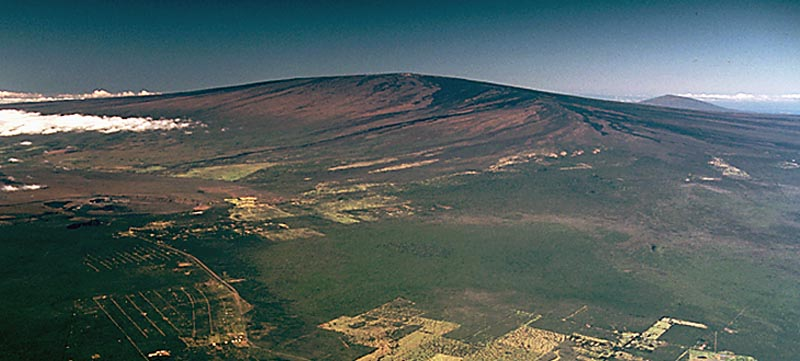
\includegraphics[width=0.8\linewidth]{images/book1/g7-mauna-loa.jpg}

{\small ماونا لوا، \omterm{def:g4:volcanoes-earthquakes-first-look:volcano}{بركان} درعي في الجزيرة الكبيرة بهاواي، كما يُرى من
الجو: \omterm{def:g1:landscapes-around-us:landform}{جبل} هائل ذو منحدرات لطيفة، بنته آلاف السيول من \omterm{def:g4:volcanoes-earthquakes-first-look:eruption}{الحمم}
السائلة. الصورة: ج.~د.~غريغز، هيئة المسح الجيولوجي الأمريكية، 1985 (ملك
عام، عبر ويكيميديا كومنز).}
% ledger: commons:mauna-loa
\label{fig:g7:volcanoes:mauna-loa}
\end{omfigure}

\section{العيش مع البراكين}

يعيش كثير من الناس قرب \omterm{def:g4:volcanoes-earthquakes-first-look:volcano}{البراكين}: فنحو 3~ملايين شخص كانوا يعيشون في المنطقة
المحيطة ببيناتوبو عام 1991. ولحسن الحظ، كثيرًا ما يعطي \omterm{def:g4:volcanoes-earthquakes-first-look:eruption}{الثوران} الكبير علامات
إنذار. \omterm{def:g7:volcanoes:magma}{فالصهارة} الصاعدة تدفع \omterm{def:g3:stones-pebbles-sand:rock}{الصخور} جانبًا: فتتشقق الأرض
وتهتز \omterm{def:g4:volcanoes-earthquakes-first-look:earthquake}{بزلازل} صغيرة، وتنتفخ المنحدرات، ويفلت الغاز. وفي \omterm{def:g1:landscapes-around-us:landform}{جبل}
سانت~هيلينز، جاءت أولى \omterm{def:g4:volcanoes-earthquakes-first-look:earthquake}{الزلازل} الصغيرة في 16~مارس 1980؛ وبحلول 17~مايو
كان قد وقع أكثر من 10\,000 \omterm{def:g4:volcanoes-earthquakes-first-look:earthquake}{زلزال}، وكان السفح الشمالي قد انتفخ نحو الخارج
بما لا يقل عن \qty{137}{m}. وقاس العلماء كل ذلك وأُغلقت
المنطقة؛ ومع ذلك، مات 57~شخصًا في 18~مايو.
% ledger: usgs:msh-lead-up, usgs:msh-flows

في بيناتوبو، عام 1991، أطلق العلماء الذين راقبوا \omterm{def:g4:volcanoes-earthquakes-first-look:earthquake}{الزلازل} والغاز
وانتفاخ \omterm{def:g4:volcanoes-earthquakes-first-look:volcano}{البركان} الإنذار في الوقت المناسب: فرحل السكان الذين يعيشون
قرب \omterm{def:g4:volcanoes-earthquakes-first-look:volcano}{البركان}، وأُنقذت حياة 5\,000 شخص على الأقل.
% ledger: usgs:pinatubo-1991 (central Luzon home to about 3 million people)

\begin{remark}[لا تقترب أبدًا من بركان ثائر]\label{rem:g7:volcanoes:safety}
مشاهدة \omterm{def:g4:volcanoes-earthquakes-first-look:eruption}{الثوران} لا تكون إلا في الأماكن التي فتحتها السلطات
للجمهور. فالغازات، \omterm{def:g3:stones-pebbles-sand:rock}{والصخور} المتساقطة، \omterm{def:g6:inside-the-earth:layers}{وقشرة} \omterm{def:g4:volcanoes-earthquakes-first-look:eruption}{الحمم} الحديثة التي تنكسر
تحت القدمين، \omterm{def:g7:volcanoes:pyroclastic-flow}{والتدفقات الفتاتية} البركانية قد تقتل، دون إنذار في الغالب.
ومراصد \omterm{def:g4:volcanoes-earthquakes-first-look:volcano}{البراكين} تنشر ما تجوز زيارته بأمان: فاتبع تعليماتها دائمًا.
\end{remark}

\section{تمارين}

\begin{exercise}[$\star$]\label{exo:g7:volcanoes:1}
صِل كل كلمة بمعناها: \omterm{def:g7:volcanoes:magma}{الصهارة}؛ \omterm{def:g4:volcanoes-earthquakes-first-look:eruption}{الحمم}؛ \omterm{def:g7:volcanoes:magma-chamber}{حجرة الصهارة}؛ \omterm{def:g7:volcanoes:vent}{المنفذ}؛
\omterm{def:g7:volcanoes:vent}{الفوهة}. (أ) تجويف على شكل وعاء في قمة \omterm{def:g4:volcanoes-earthquakes-first-look:volcano}{البركان}. (ب) \omterm{def:g3:stones-pebbles-sand:rock}{صخر} منصهر
تحت الأرض. (ج) فتحة تخرج منها \omterm{def:g7:volcanoes:magma}{الصهارة}. (د) \omterm{def:g3:stones-pebbles-sand:rock}{صخر} منصهر
خرج إلى السطح. (ه) جيب كبير من \omterm{def:g7:volcanoes:magma}{الصهارة} على بعد بضعة
كيلومترات تحت \omterm{def:g4:volcanoes-earthquakes-first-look:volcano}{البركان}.
\end{exercise}

\begin{exercise}[$\star$]\label{exo:g7:volcanoes:2}
انسيابي أم انفجاري؟ (أ) \omterm{def:g1:landscapes-around-us:water}{أنهار} من \omterm{def:g4:volcanoes-earthquakes-first-look:eruption}{الحمم} المتوهجة تجري على منحدر
لطيف. (ب) عمود من الرماد يرتفع \qty{35}{km} في السماء. (ج)
نافورة من القطرات المتوهجة تندفع من شق. (د) انهيار من الرماد الحار
والغاز يندفع في \omterm{def:g1:landscapes-around-us:landform}{وادٍ}.
\end{exercise}

\begin{exercise}[$\star$]\label{exo:g7:volcanoes:3}
صواب أم خطأ؟ صحّح الجمل الخاطئة. (أ) \omterm{def:g7:volcanoes:magma}{الصهارة} \omterm{def:g4:volcanoes-earthquakes-first-look:eruption}{والحمم} اسمان
\omterm{def:g3:stones-pebbles-sand:rock}{للصخر} المنصهر نفسه، تحت الأرض وعلى السطح. (ب) أوفر
الغازات البركانية هو ثاني أكسيد الكربون. (ج) \omterm{def:g7:volcanoes:pyroclastic-flow}{التدفق الفتاتي البركاني} \omterm{def:g1:landscapes-around-us:water}{نهر}
من \omterm{def:g4:volcanoes-earthquakes-first-look:eruption}{الحمم} السائلة. (د) \omterm{def:g4:volcanoes-earthquakes-first-look:volcano}{براكين} هاواي تقع على \omterm{def:g7:plate-tectonics:plate-boundary}{حد صفائح}.
\end{exercise}

\begin{exercise}[$\star$]\label{exo:g7:volcanoes:4}
استعمل جدول ألوان التوهج. (أ) \omterm{def:g4:volcanoes-earthquakes-first-look:eruption}{حمم} تتوهج بالأصفر: أعطِ
درجة حرارتها. (ب) سيل \omterm{def:g4:volcanoes-earthquakes-first-look:eruption}{حمم} يتصلب يتوهج بالأحمر الداكن: أعطِ درجة حرارته.
(ج) تُظهر صورة \omterm{def:g4:volcanoes-earthquakes-first-look:eruption}{حممًا} برتقالية في مقدمة سيل \omterm{def:g4:volcanoes-earthquakes-first-look:eruption}{وحممًا} صفراء
قرب \omterm{def:g7:volcanoes:vent}{المنفذ}. أين تكون الحرارة أعلى؟ لماذا؟
\end{exercise}

\begin{exercise}[$\star\star$]\label{exo:g7:volcanoes:5}
استعمل المخطط العمودي \omterm{def:g4:volcanoes-earthquakes-first-look:volcano}{للبراكين} البالغ عددها 1\,214. (أ) كم \omterm{def:g4:volcanoes-earthquakes-first-look:volcano}{بركانًا} يقع على
\omterm{def:g7:plate-tectonics:plate-boundary}{حد صفائح} (حيث تتباعد \omterm{def:g7:plate-tectonics:plate}{الصفائح}، أو حيث تغوص \omterm{def:g7:plate-tectonics:plate}{صفيحة} تحت
أخرى)؟ (ب) ما النسبة المئوية التي يمثلها ذلك من كل \omterm{def:g4:volcanoes-earthquakes-first-look:volcano}{البراكين}؟ (ج) تحقق من أن
مجموع النسب المئوية الأربع في القضية يساوي نحو 100~\%.
\end{exercise}

\begin{exercise}[$\star\star$]\label{exo:g7:volcanoes:6}
من بين المخاريط الشديدة الانحدار (\omterm{def:g4:volcanoes-earthquakes-first-look:volcano}{البراكين} الطبقية) في القائمة، وعددها 660، يقع 564 حيث تغوص
\omterm{def:g7:plate-tectonics:plate}{صفيحة} تحت أخرى، و62 حيث تتباعد \omterm{def:g7:plate-tectonics:plate}{الصفائح}، و33 داخل
\omterm{def:g7:plate-tectonics:plate}{صفيحة}. (أ) أوجد النسبة المئوية للمخاريط الشديدة الانحدار الواقعة حيث تغوص \omterm{def:g7:plate-tectonics:plate}{صفيحة}
تحت أخرى. (ب) كم مخروطًا شديد الانحدار يبقى للموقع «غير
المعروف»؟ (ج) استعمل الأدلة الأربعة: ما نوع \omterm{def:g4:volcanoes-earthquakes-first-look:eruption}{الثورانات} التي نتوقعها
على طول حزام النار؟
\end{exercise}

\begin{exercise}[$\star\star$]\label{exo:g7:volcanoes:7}
في كيلاويا، تغادر \omterm{def:g4:volcanoes-earthquakes-first-look:eruption}{الحمم} \omterm{def:g7:volcanoes:vent}{المنفذ} وحرارتها نحو \qty{1170}{\degreeCelsius}. وفي
نفق \omterm{def:g4:volcanoes-earthquakes-first-look:eruption}{حمم} بلغت \omterm{def:g2:water-on-earth:ocean}{البحر}، على بعد \qty{10}{km}، وحرارتها نحو
\qty{1140}{\degreeCelsius}. (أ) بكم درجة بردت؟ (ب) كم
درجة يساوي ذلك لكل كيلومتر؟ (ج) \omterm{def:g4:volcanoes-earthquakes-first-look:eruption}{الحمم} في الهواء الطلق تبرد بمئات
الدرجات في الثانية عند سطحها. اشرح لماذا بقيت \omterm{def:g4:volcanoes-earthquakes-first-look:eruption}{الحمم} في
النفق حارة إلى هذا الحد.
\end{exercise}

\begin{exercise}[$\star\star$]\label{exo:g7:volcanoes:8}
أقدم \omterm{def:g3:stones-pebbles-sand:rock}{صخور} كاواي عمرها نحو 5.5~مليون سنة؛ \omterm{def:g3:stones-pebbles-sand:rock}{وصخور} الجزيرة
الكبيرة عمرها أقل من 0.7~مليون سنة. (أ) أي الجزيرتين أقدم؟ وبكم مليون سنة على
الأقل؟ (ب) أي الجزيرتين أشد تآكلًا؟ لماذا؟
(ج) أي الجزيرتين تقع فوق \omterm{def:g7:volcanoes:hotspot}{البقعة الساخنة} اليوم؟ (د) تقع كاواي شمال غرب
الجزيرة الكبيرة. في أي اتجاه تحمل \omterm{def:g7:plate-tectonics:plate}{صفيحة} \omterm{def:g2:water-on-earth:ocean}{المحيط} الهادئ
الجزر؟
\end{exercise}

\begin{exercise}[$\star\star$]\label{exo:g7:volcanoes:9}
تقع جزر هاواي على بعد أكثر من \qty{3200}{km} من أقرب \omterm{def:g7:plate-tectonics:plate-boundary}{حد
صفائح}. (أ) لماذا يُعد ذلك مفاجئًا بالنسبة إلى \omterm{def:g4:volcanoes-earthquakes-first-look:volcano}{البراكين}؟ (ب) اشرح في ثلاث أو
أربع جمل من أين تأتي صهارتها. (ج) على \omterm{def:g2:drawing-to-map:map}{خريطة}
\omterm{def:g4:volcanoes-earthquakes-first-look:volcano}{البراكين}، ما لونها؟
\end{exercise}

\begin{exercise}[$\star\star$]\label{exo:g7:volcanoes:10}
في يونيو~1991 نزّت أول \omterm{def:g7:volcanoes:magma}{صهارة} من بيناتوبو بهدوء؛ وبعد ثلاثة أيام،
انفجرت \omterm{def:g7:volcanoes:magma}{صهارة} أخرى. مستعينًا بقنينتي الماء الغازي، اشرح
الفرق. أي الصهارتين كانت قد فقدت غازها في طريقها إلى الأعلى؟
\end{exercise}

\begin{exercise}[$\star\star\star$]\label{exo:g7:volcanoes:11}
تقع قرية على بعد \qty{10}{km} أسفل \omterm{def:g1:landscapes-around-us:landform}{وادٍ} ينحدر من \omterm{def:g4:volcanoes-earthquakes-first-look:volcano}{بركان}. (أ)
يتحرك \omterm{def:g7:volcanoes:pyroclastic-flow}{تدفق فتاتي بركاني} بسرعة \qty{80}{km/h}. كم دقيقة يستغرق
ليصل إلى القرية؟ (ب) السؤال نفسه بسرعة \qty{130}{km/h}. (ج) تحتاج أسرة
إلى 20~دقيقة لترحل بالسيارة. اشرح لماذا يجب أن يأتي الإنذار
قبل بدء \omterm{def:g4:volcanoes-earthquakes-first-look:eruption}{الثوران}، لا حين يُرى التدفق.
\end{exercise}

\begin{exercise}[$\star\star\star$]\label{exo:g7:volcanoes:12}
دار رماد \omterm{def:g1:landscapes-around-us:landform}{جبل} سانت~هيلينز حول الأرض كلها مرة واحدة في 15~يومًا.
\omterm{def:g6:latitude-longitude:latitude}{ودرجة العرض} الواحدة نحو \qty{111}{km}، والدورة الكاملة
360~درجة. (أ) ما الطول التقريبي لدورة كاملة حول الأرض، بالكيلومترات؟
قرّب إلى أقرب ألف. (ب) كم كيلومترًا قطع
الرماد في اليوم، في المتوسط؟ (ج) كم كيلومترًا في الساعة يساوي
ذلك؟ (د) هل تحمل الريحُ الرمادَ أم ينتقل بسرعته الخاصة؟ اشرح.
% ledger: usgs:msh-may18, rmg:latitude-def
\end{exercise}

\section{مسألة: اليوم الذي فقد فيه الجبل قمته}

\begin{problem}[{مسألة نهاية الأسبوع --- علامات الإنذار في جبل سانت~هيلينز،
وثوران 18~مايو 1980، وكم فُقد من الجبل}]
\label{pb:g7:volcanoes:1}
% ledger: usgs:msh-heights, usgs:msh-lead-up, usgs:msh-may18, usgs:msh-flows, usgs:msh-reach, usgs:msh-dome, usgs:msh-faq-loss, data:gvp, tht:everest

يقع \omterm{def:g1:landscapes-around-us:landform}{جبل} سانت~هيلينز في الشمال الغربي من الولايات المتحدة. استعمل
الصورتين في أول الفصل، \omterm{def:g2:drawing-to-map:map}{وخريطة} \omterm{def:g4:volcanoes-earthquakes-first-look:volcano}{البراكين}، والأعداد
أدناه، التي قاستها هيئة المسح الجيولوجي الأمريكية.

\medskip
\noindent\textbf{الجزء الأول --- قبل الثوران.}
\begin{enumerate}
  \item جاءت أولى \omterm{def:g4:volcanoes-earthquakes-first-look:earthquake}{الزلازل} الصغيرة في 16~مارس 1980؛ \omterm{def:g4:volcanoes-earthquakes-first-look:eruption}{والثوران}
        الكبير في 18~مايو. كم يومًا مر بين الحدثين؟ (في مارس
        31~يومًا، وفي أبريل~30.)
  \item بحلول 17~مايو، كان قد سُجّل أكثر من 10\,000 \omterm{def:g4:volcanoes-earthquakes-first-look:earthquake}{زلزال}،
        خلال 62~يومًا منذ 16~مارس. فكم \omterm{def:g4:volcanoes-earthquakes-first-look:earthquake}{زلزالًا} يساوي ذلك تقريبًا في اليوم، في
        المتوسط؟
  \item انتفخ السفح الشمالي \omterm{def:g1:landscapes-around-us:landform}{للجبل} نحو الخارج بما لا يقل عن
        \qty{137}{m}. اشرح لماذا أقلق الانتفاخ العلماء.
  \item على \omterm{def:g2:drawing-to-map:map}{خريطة} \omterm{def:g4:volcanoes-earthquakes-first-look:volcano}{البراكين}، \omterm{def:g1:landscapes-around-us:landform}{جبل} سانت~هيلينز مثلث أزرق.
        ماذا يخبرك ذلك عن موقعه؟ وأي نوع من \omterm{def:g4:volcanoes-earthquakes-first-look:eruption}{الثوران}
        تتوقع، وأي شكل \omterm{def:g4:volcanoes-earthquakes-first-look:volcano}{للبركان}؟
\end{enumerate}

\medskip
\noindent\textbf{الجزء الثاني --- 18 مايو 1980.}\par\nopagebreak
\begin{enumerate}[resume, beginpenalty=10000]
  \item في الساعة \babelsublr{8:32} جعل \omterm{def:g4:volcanoes-earthquakes-first-look:earthquake}{زلزال} صغير السفح المنتفخ ينزلق.
        وتحرك \omterm{def:g5:natural-hazards:landslide}{الانزلاق الأرضي} بسرعة بلغت \qty{240}{km/h}. فكم كيلومترًا
        يساوي ذلك في الدقيقة؟
  \item كشف \omterm{def:g5:natural-hazards:landslide}{الانزلاق الأرضي} \omterm{def:g7:volcanoes:magma}{الصهارة} كسدادة تُنزع من قنينة
        مرجوجة. اشرح لماذا انفجر \omterm{def:g4:volcanoes-earthquakes-first-look:volcano}{البركان} عندئذ جانبيًا.
  \item تحرك الانفجار الجانبي بسرعة لا تقل عن \qty{480}{km/h} ووصل إلى
        \qty{27}{km} من \omterm{def:g4:volcanoes-earthquakes-first-look:volcano}{البركان}. بهذه السرعة، كم دقيقة استغرق
        على الأكثر ليصل إلى هناك؟
  \item تحركت \omterm{def:g7:volcanoes:pyroclastic-flow}{التدفقات الفتاتية} البركانية بسرعة بلغت \qty{130}{km/h} ووصلت إلى
        \qty{8}{km} من \omterm{def:g7:volcanoes:vent}{الفوهة}. كم دقيقة استغرقت بتلك
        السرعة؟ قرّب إلى أقرب دقيقة.
\end{enumerate}

\medskip
\noindent\textbf{الجزء الثالث --- بعد الثوران.}\par\nopagebreak
\begin{enumerate}[resume, beginpenalty=10000]
  \item بلغ عمود الرماد \omterm{def:g4:world-physical-map:altitude}{ارتفاع} نحو \qty{24}{km} في أقل
        من 15~دقيقة. كم مرة يعادل ذلك \omterm{def:g4:world-physical-map:altitude}{ارتفاع} \omterm{def:g1:landscapes-around-us:landform}{جبل} إفرست
        (\qty{8.8}{km})؟ قرّب إلى منزلة عشرية واحدة.
  \item بين عامي 1980 و1986، نزّت \omterm{def:g4:volcanoes-earthquakes-first-look:eruption}{حمم} لزجة في \omterm{def:g7:volcanoes:vent}{الفوهة}
        وبنت كومة ارتفاعها \qty{267}{m} فوق \omterm{def:g7:volcanoes:vent}{المنفذ}. هل كانت هذه
        \omterm{def:g4:volcanoes-earthquakes-first-look:eruption}{الثورانات} انسيابية أم انفجارية؟ وأي قنينة من قنينتي الماء الغازي
        تذكّرك بها؟
  \item انظر إلى صورتي \omterm{def:g4:volcanoes-earthquakes-first-look:volcano}{البركان}. صِف في
        جملتين ما الذي تغيّر.
  \item قبل \omterm{def:g4:volcanoes-earthquakes-first-look:eruption}{الثوران}، كانت القمة على \omterm{def:g4:world-physical-map:altitude}{ارتفاع} \qty{2950}{m} فوق \omterm{def:g4:world-physical-map:altitude}{مستوى سطح البحر}؛
        وبعده، صارت أعلى نقطة على \omterm{def:g4:world-physical-map:altitude}{ارتفاع} \qty{2549}{m}. كم مترًا من
        \omterm{def:g4:world-physical-map:altitude}{الارتفاع} فقد \omterm{def:g1:landscapes-around-us:landform}{الجبل}؟
\end{enumerate}
\end{problem}
